\chapter{Experiments and Results}
\thispagestyle{plain}
\label {Experiments and Results}

In this chapter we discuss the datasets used and the experiment setup to test the column separation, column annotations and relation predictions. We also evaluate the framework as we explain the results from the various experiments performed on the datasets.


\section{Data Setup}
We use different sets of log files to test the framework. Primarily, we use two datasets viz., original log files and synthetically generated log files. Table~\ref{table:dataset_distribution} gives a general statistic about the log files in each dataset, total columns, average columns and relations per table in all the log files of the dataset.

\newcommand{\specialcell}[2][c]{%
  \begin{tabular}[#1]{@{}c@{}}#2\end{tabular}}

\begin{table}[htbp]
\caption{Number of log files, total columns present, average columns and relations per table in each dataset}
\bigskip
\label{table:dataset_distribution}
\centering
\begin{center}
\def\arraystretch{1.8}
\begin{tabular}{|@{\hskip 1cm}c@{\hskip 1cm}|c|c|c|c|}
\hline
\textit{Dataset} & \textit{Tables} & \textit{Columns} & \specialcell{\textit{Average Columns/} \\ \textit{Table}} & \specialcell{\textit{Average Relations/}\\ \textit{Table}} \\
\hline
Original & 11 & 78 & 7 & 3 \\
\hline
Synthetic & 20 & 150 & 8 & 5 \\
\hline
\end{tabular}
\end{center}
\end{table}

The Original dataset contains actual log files as obtained from various tools and services running in an operating system. This includes \textit{Linux} system services like syslog, kern, auth, etc. We also have log files from commonly used services like apache2, mongodb, sendmail, printers, etc.
\\

The Synthetic dataset has a set of artificially generated log files using some known columns. These columns are generally seen in log files like those present in the Original dataset. The synthetic log files were generated to test the framework against log files with unknown source and format.

To create these synthetic log files, we randomized the whole process. The number of columns in every log file was randomly chosen. Later, we arbitrarily selected the type of columns from the manually prepared superset of columns. While generating the columns we probabilistically added different column values to the selected columns. This noise was added to simulate unpredictable nature of log files. Also, all the values added in the columns for a particular type were generated at random to ensure variation in length and other properties of the column.


\section{Tabulation}

In this experiment we tested the precision with which the log files are converted into tables with proper set of columns. The \textit{Tabulate} module of the framework, splits the log file to convert it into a table. This is a simple test where we have log files with separable columns. We feed these log files to the \textit{Tabulate} module and get an output table with certain set of columns. We try and match all the output columns to the expected sample. Thus, we not only check the number of columns separated we also check the exact boundaries of separation.

\begin{figure}[h]
	\centering
	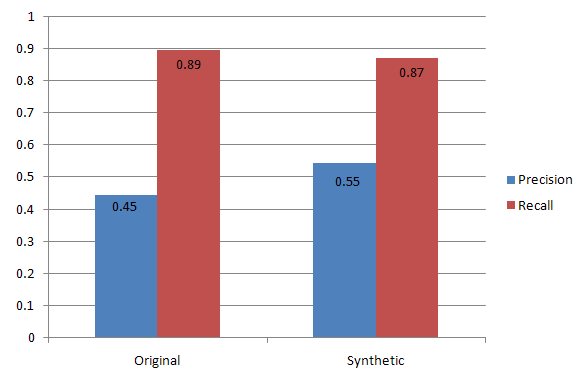
\includegraphics[width=0.9\textwidth, height=0.5\textheight, keepaspectratio] {tabulate_precision_recall_1.png}
	\caption{Precision and recall for column separation}
	\label{fig:tabulate_precision_recall_1}
\end{figure}

As discussed in previous chapter, we separate the log files using standard delimiters. Due to this, columns with multiple words but no surrounding characters, get separated as multiple columns in our framework. It is observed, that in most of the cases such descriptive columns with multiple words are found at the tail of the log entry. Thus, most of the initial columns are easily separated. Due to the said fact about log files, our framework can give out more columns than the expected number of columns. We gets a high recall as we do not expect those columns to be separated. While the recall is high, we observe a low precision. Due to the extraneous columns, which are not there in the original log files, we get a low precision compared to the recall. In Figure~\ref{fig:tabulate_precision_recall_1} we see that for both the datasets, we get a high recall and low precision.

\begin{figure}[h]
	\centering
	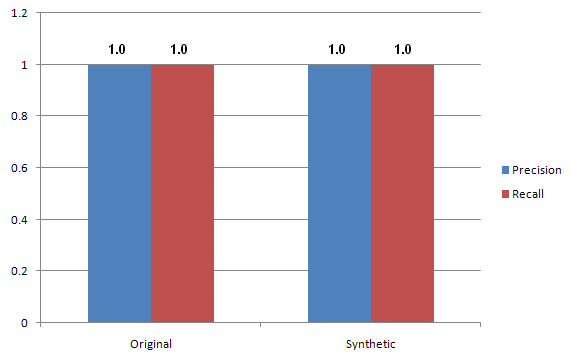
\includegraphics[width=0.9\textwidth, height=0.5\textheight, keepaspectratio] {tabulate_precision_recall_2.png}
	\caption{Precision and recall for column separation without trailing textual data}
	\label{fig:tabulate_precision_recall_2}
\end{figure}

We repeat this experiment with the same log files, but now we strip out the trailing textual part. In real life, we can find tools which can clean the log files and in this case strip the unwanted text. Figure~\ref{fig:tabulate_precision_recall_2} shows the precision and recall with the modified log files. Now, we see that both precision and recall are high for the datasets. The high
precision in the later case indicates that most of the log files have structured data at the beginning of the log entries and is followed by a more verbose message field.

Although the recall of both the datasets is almost similar, we see that it is slightly better in the Original dataset (Figure~\ref{fig:tabulate_precision_recall_1}). Some of the log files like \textit{apache\_access} have the textual part embedded in quotes. This makes it easier for the \textit{Tabulate} module to separate the column as a whole. While in the Synthetic dataset, we have appended the text without enclosing quotes. Hence, the recall is better in the Original dataset compared to the Synthetic dataset.


\section{Column Annotation}

\begin{figure}[h]
	\centering
	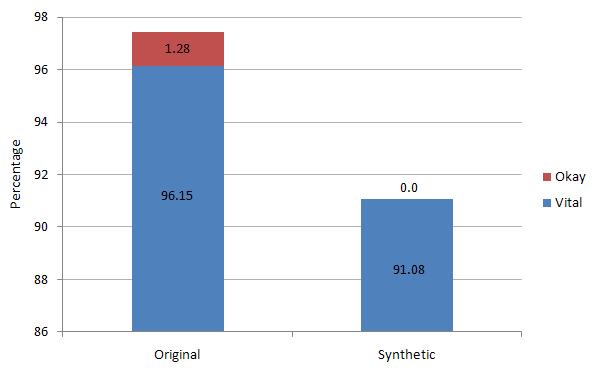
\includegraphics[width=0.9\textwidth, height=0.5\textheight, keepaspectratio] {decode_rank_1_partial.png}
	\caption{Percentage of \textit{vital} and \textit{okay} classes at rank 1}
	\label{fig:decode_rank_1_partial}
\end{figure}

In the \textit{Decode} module we annotate the columns present in the table generated by the \textit{Tabulate} module. We gave columns from the log files to manual annotators. The annotations from the manual annotators form the ground truth for this module. The manual annotators mark each class as \textit{vital}, \textit{okay} or \textit{incorrect}, for every column in the table. This is analogous to the strategy adopted by Venetis \textit{et al}.\cite{venetis2011recovering}. For instance, an annotator could mark, the \textit{URL} class as \textit{vital}, \textit{FilePath} as \textit{okay} and \textit{HTTPMethod} as \textit{incorrect}, for the column \textit{URL}. Each column may have multiple \textit{vital}, \textit{okay} or \textit{incorrect} labels. This task of manual annotation was given to three Graduate students in Computer Science at the University of Maryland, Baltimore County.

The human annotators were given ten classes for every column. If they could not match the column to any of the known ten classes, they would mark it as \textit{No Annotation} (N.A.). Even in our framework we marked N.A. for the columns that were not recognizable by the system. We considered the column annotation to be accurate if both the human annotator and the framework gave \textit{No Annotation}.

\begin{figure}[h]
	\centering
	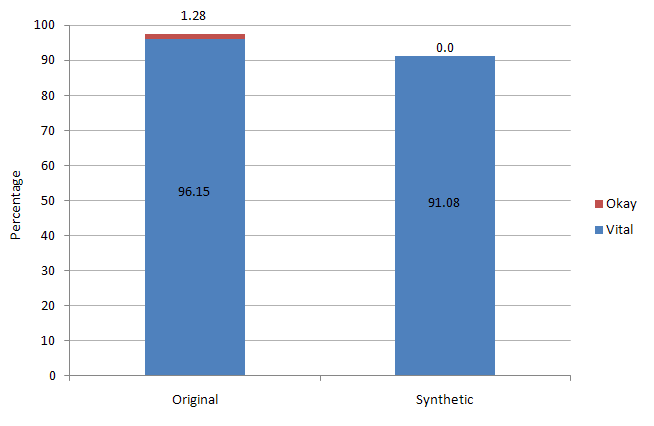
\includegraphics[width=0.9\textwidth, height=0.5\textheight, keepaspectratio] {decode_rank_1_full.png}
	\caption{Percentage of \textit{vital} and \textit{okay} classes at rank 1}
	\label{fig:decode_rank_1_full}
\end{figure}

In the \textit{Decode} module, we get a ranked list of classes for every column in the table. Figure~\ref{fig:decode_rank_1_partial}, shows the percentage distribution of \textit{vital} and \textit{okay} classes found at rank 1. This is an aggregate of all the columns in the datasets. In the Original dataset, 96.15\% of the top ranked class labels are marked as \textit{vital} and 1.28\% are marked as \textit{okay}. While in the Synthetic dataset, 91.08\% of the top ranked class labels are marked as \textit{vital}. There are no top ranked class labels marked as \textit{okay}. Thus, the distribution is highly inclined towards \textit{vital} for columns in both the datasets. 

Figure~\ref{fig:decode_rank_1_full} shows the zoomed out version of Figure~\ref{fig:decode_rank_1_partial}. It is observed that there is not much difference in the percentage of correctly predicted classes for both datasets. Overall we see a good percentage of relevant class labels, i.e., either \textit{vital} or \textit{okay}, are found at rank 1. Thus, the system has a good accuracy for column prediction as most of the predicted class labels are found at the topmost rank.

\begin{figure}[h]
	\centering
	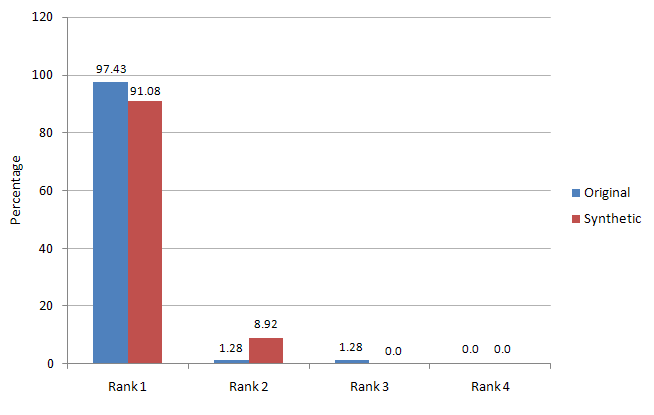
\includegraphics[width=\textwidth, height=\textheight, keepaspectratio] {decode_rank_1_to_4.png}
	\caption{Percentage of relevant classes at ranks 1 to 4}
	\label{fig:decode_all_rank_acccuracy}
\end{figure}

Figure~\ref{fig:decode_all_rank_acccuracy} shows the distribution of relevant class labels at different ranks in the system. As concluded from Figure~\ref{fig:decode_rank_1_partial}, we can see that most of the relevant class labels are found at rank 1. Very few relevant class labels are found at ranks 2 and 3. It is observed that none of the lower ranks from 4 have the relevant class labels. Due to the almost structured nature of the log file, we get a lot of rows with appropriate column values, leading to proper annotation of the column.

Also, the relevant class labels for both the datasets are comparable. We see that percentage of relevant class labels at rank 1 are slightly less for Synthetic dataset. This is because columns like \textit{URL} are sometimes also classified as \textit{FilePath}. This causes the \textit{URL} class label to be at rank 2. There are more such columns in the Synthetic dataset due to our probabilistic approach of log file generation.


\section{Relation Annotation}

Similar to the \textit{Decode} module we annotate the relations between various columns present in the table. These relations are predicted using the IDS Ontology. We gave tabulated log files to human annotators, and they were asked to annotate the relation for a set of column pairs in them. For every pair of columns they were given a set a relation labels. The annotators marked each relation label as \textit{vital}, \textit{okay} or \textit{incorrect}, for every pair of columns given to them. This is again, similar to the strategy used by Venetis \textit{et al.}\cite{venetis2011recovering}. The annotators were allowed to mark multiple labels as \textit{vital}, \textit{okay} or \textit{incorrect}. They were given a choice to mark a relation as No Annotation (N.A.) if they did not find suitable relation from the given set of relation labels.

Figure~\ref{fig:relation_precision_recall} shows the precision and recall calculated for the relation prediction module. It is observed that the recall for both datasets is very high. The relations that are predicted by our framework come out to be accurate, and hence we get a very high recall. While the precision of the Original dataset is very high, that of the Synthetic dataset comes out quite less comparatively. Most of the relationships we have in the ontology are added by observing the actual log files present in the Original dataset. That is why, our framework's predictions match quite well with the actual relations. On the other hand, in Synthetic dataset, there are a lot of false positives. This means we are predicting relations that do not exist in the human annotated source. Hence, we see a dip in the precision of relation prediction for Synthetic dataset.

\begin{figure}[h]
	\centering
	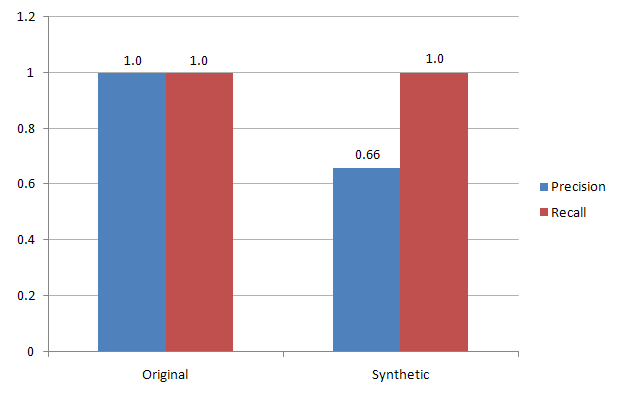
\includegraphics[width=0.9\textwidth, height=\textheight, keepaspectratio] {relation_precision_recall.png}
	\caption{Precision and recall for relation annotations}
	\label{fig:relation_precision_recall}
\end{figure}

Figure~\ref{fig:relation_vital_okay_partial} shows the percentage distribution of predicted relations that are marked as \textit{vital} and \textit{okay}. Almost all of the relations predicted are annotated as \textit{vital} by the human annotators. In the Original dataset all the predicted relations are annotated as \textit{vital}. While in Synthetic dataset, a small percentage i.e. 6.67\% of predicted relations are marked as \textit{okay} and rest are \textit{vital}. There are pairs of column like \textit{EmailAddress} and \textit{Timestamp} that have multiple relations like \textit{sentAt} and \textit{receivedAt} amongst them. This causes some of them to be marked as \textit{okay} by human annotators. Such pairs occur more frequently in the Synthetic dataset and hence it has higher percentage of \textit{okay} labels compared to the Original dataset. Figure~\ref{fig:relation_vital_okay_full} is a zoomed out version of Figure~\ref{fig:relation_vital_okay_partial}. It clearly shows that there is not much difference in the distribution of \textit{vital} and \textit{okay} labels for both datasets. Also, most of predicted relations are marked as \textit{vital}.


\begin{figure}[h]
	\centering
	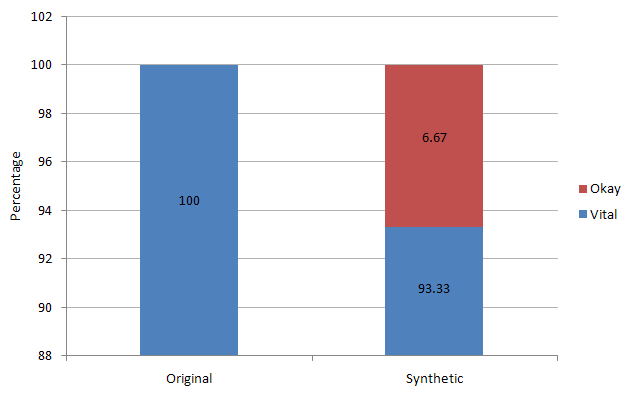
\includegraphics[width=0.9\textwidth, height=\textheight, keepaspectratio] {relation_vital_okay_partial.png}
	\caption{Percentage of \textit{vital} and \textit{okay} relation labels}
	\label{fig:relation_vital_okay_partial}
\end{figure}

\begin{figure}[h]
	\centering
	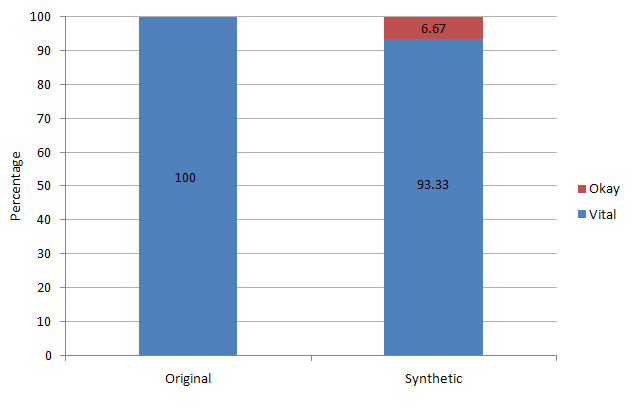
\includegraphics[width=0.9\textwidth, height=\textheight, keepaspectratio] {relation_vital_okay_full.png}
	\caption{Percentage of \textit{vital} and \textit{okay} relation labels}
	\label{fig:relation_vital_okay_full}
\end{figure}




